\documentclass[a4paper,12pt]{article}
\usepackage[T1]{fontenc}
\usepackage[utf8]{inputenc}
\usepackage{tikz}
\usepackage{graphicx}
\usepackage{amsmath}
\usepackage{geometry}
\geometry{margin=2cm}

\title{LABORATORY07: Report and Presentation of work on Beamer and Posters}
\author{PELE TETE\RUDN}
\date{December 2025}

\begin{document}

\maketitle
\tableofcontents
\newpage

% ============================================================
\section{700IntroductionBeamer - Basic Beamer Presentation}
\label{sec:700}

\begin{verbatim}
\documentclass{beamer}
\usetheme{Copenhagen}

\title{Présentation Beamer}
\author{PELE TETE}
\date{01 01 2025}

\begin{document}

\begin{frame}
\titlepage
\end{frame}

\begin{frame}
\frametitle{Introduction}
\begin{itemize}
\item COMMENT UTILISER BEAMER
\item COMMENT JE PEUX REUSSIR LES LABO DE KOULYABOV
\item COMMENT DOIS-JE REDIGER LES LABO DE KOULYABOV
\end{itemize}
\end{frame}

\begin{frame}
\frametitle{Méthodologie}
\begin{block}{Étapes de la méthode}
1. Préparation des labo\\
2. Analyse et lecture du livre\\
3. Compillation des codes-exemples et autres codes
\end{block}
\end{frame}

\begin{frame}
\frametitle{Résultats}
\begin{columns}
\begin{column}{0.5\textwidth}
\begin{itemize}
\item Résultat des labo
\item Résultat des retenus de la lecture
\item Résultat des compillations des codes
\end{itemize}
\end{column}
\begin{column}{0.5\textwidth}
\includegraphics[width=\textwidth]{faucon.jpg}
\end{column}
\end{columns}
\end{frame}

\begin{frame}
\frametitle{Conclusion}
\begin{alertblock}{Points clés}
\begin{itemize}
\item Conclusion principale
\item Implications pratiques
\item Directions futures
\end{itemize}
\end{alertblock}
\end{frame}

\end{document}
\end{verbatim}

\subsection*{Generated figure (simulation)}
Beamer presentation with title page, introduction, methodology, results, and conclusion slides.

\subsection*{Imported image}
\begin{center}
\includegraphics[width=0.8\textwidth]{700IntroductionBeamer.png}
\end{center}

\vspace{20pt}\hrule\vspace{20pt}

% ============================================================
\section{711StructureOfApresentation - Basic Beamer Structure}
\label{sec:711}

\begin{verbatim}
\documentclass{beamer}% use of beamer 

\usetheme{Copenhagen}
\author{Bert}
\title{A tale of two primes}

\begin{document}
All is good
\end{document}
\end{verbatim}

\subsection*{Generated figure (simulation)}
Minimal Beamer document structure.

\subsection*{Screenshot}
\begin{center}
\includegraphics[width=0.8\textwidth]{711StructureOfApresentation.png}
\end{center}

\vspace{20pt}\hrule\vspace{20pt}

% ============================================================
\section{712BeamerFrame - Basic Frame Usage}
\label{sec:712}

\begin{verbatim}
\documentclass{beamer}
\begin{document}
\usetheme{Copenhagen}
\author{Bert}
\title{A tale of two primes}

\begin{frame}% use of  frame (in beginner)
\titlepage
\end{frame}% use of  frame (at the end)
\begin{frame}{Article}% use of  frame (in beginner)
Some text about the article.
\end{frame}% use of  frame (at the end)
\begin{frame}{Mathematica}%use of  frame (in beginner)
A helpful tool for mathematicians.
\end{frame}% use of  frame (at the end)

\end{document}
\end{verbatim}

\subsection*{Generated figure}
Beamer presentation with title page and two content frames.

\subsection*{Screenshot}
\begin{center}
\includegraphics[width=0.6\textwidth]{712BeamerFrame.png}
\end{center}

\vspace{20pt}\hrule\vspace{20pt}

% ============================================================
\section{712BeamerFrame2 - Blocks in Frames}
\label{sec:712b}

\begin{verbatim}
\documentclass{beamer}
\begin{document}
\usetheme{Copenhagen}
\author{Bert}
\title{A tale of two primes}

\begin{frame}{Article}
\begin{block}{Example}
This is an example of a block.
\end{block}
\begin{block}{Euclid's theorem}
This is a theorem.
\end{block}
\end{frame}

\end{document}
\end{verbatim}

\subsection*{Generated figure}
Frame with example and theorem blocks.

\subsection*{Screenshot}
\begin{center}
\includegraphics[width=0.6\textwidth]{712BeamerFrame2.png}
\end{center}

\vspace{20pt}\hrule\vspace{20pt}

% ============================================================
\section{713BeamerFramePause - Pausing Between Blocks}
\label{sec:713}

\begin{verbatim}
\documentclass{beamer}
\begin{document}
\usetheme{Copenhagen}
\author{Bert}
\title{A tale of two primes}

\begin{frame}{Article}
\begin{block}{Definition}
This is a definition.
\end{block}
\pause% use of pause to get one by one the slide
\begin{block}{Euclid's theorem}
This is a theorem.
\end{block}
\end{frame}

\end{document}
\end{verbatim}

\subsection*{Generated figure}
Frame with pause between blocks.

\subsection*{Screenshot}
\begin{center}
\includegraphics[width=0.6\textwidth]{713BeamerFramePause.png}
\end{center}

\vspace{20pt}\hrule\vspace{20pt}

% ============================================================
\section{713BeamerFramePauseEnumerate - Pause with Enumerate}
\label{sec:713b}

\begin{verbatim}
\documentclass{beamer}
\begin{document}
\usetheme{Copenhagen}
\author{Bert}
\title{A tale of two primes}

\begin{frame}{Title}
\begin{enumerate} %use of pause and  enumerate in order to enumerate
\item Element
\pause%use of the pause for the slide
\item Element
\pause%use of the pause for the slide
\item Element
\end{enumerate}%use of pause and  enumerate in order to enumerate
\end{frame}
\end{document}
\end{verbatim}

\subsection*{Generated figure}
Enumerated list with pauses.

\subsection*{Screenshot}
\begin{center}
\includegraphics[width=0.6\textwidth]{713BeamerFramePauseEnumerate.png}
\end{center}

\vspace{20pt}\hrule\vspace{20pt}

% ============================================================
\section{720Uncover - Basic Uncover Command}
\label{sec:720}

\begin{verbatim}
\documentclass{beamer}
\begin{document}
\usetheme{Copenhagen}
\author{Bert}
\title{A tale of two primes}
%We are going to see how by using \uncover, we can determine when each part of the slide will appear
\begin{frame}
\frametitle{Sets}
A \verb|\alert{set}| is a collection of objects.\verb|\uncover<2->|{ For example:

\[
Z=\{\text{cow},\text{pig},\text{elephant}\}.}
\]
\uncover<3->{We call the objects in $Z$ the \alert{elements} of $Z$.}\uncover<4->{ We write
\[
\text{cow} \in Z
\]}
\uncover<5->{with \`\`cow is an element of $Z$''.}\uncover<6->{ Frequently encountered sets are}

\[
\begin{split}
\uncover<7->{\mathbb{N}} \uncover<8->{= \{1,2,3,\ldots \}}&\uncover<9->{ \qquad (\text{\`\`natural numbers''})\\}
\uncover<10->{\mathbb{Z}} \uncover<11->{= \{\ldots,-2,-1,0,1,2,\ldots \}}&\uncover<12->{ \qquad (\text{\`\`integer numbers''})\\}
\uncover<13->{\mathbb{Q}} \uncover<14->{= \{p/q : p,q\in\mathbb{Z} \text{ and } q\neq 0\} }&\uncover<15->{\qquad (\text{\`\`rational numbers''})\\}
\uncover<16->{\mathbb{R}} \uncover<17->{= \{\hbox{decimal numbers}\}}&\uncover<18->{\quad\qquad (\text{\`\`real numbers''})}
\end{split}
\]
\end{frame}
\end{document}
\end{verbatim}

\subsection*{Generated figure}
Step-by-step revelation of set definitions.

\subsection*{Screenshot}
\begin{center}
\includegraphics[width=0.7\textwidth]{720Uncover.png}
\end{center}

\vspace{20pt}\hrule\vspace{20pt}

% ============================================================
\section{720UncoverInAlign2 - Uncover in Align Environment}
\label{sec:720a}

\begin{verbatim}
\documentclass{beamer}
\begin{document}
\usetheme{Copenhagen}
\author{Bert}
\title{A tale of N primes}
%We can also use \uncover in the align environment.
\begin{frame}
     The derivative of $f(x) = g(x) \cdot h(x)$, with $g(x) = x^2$ and $h(x) = \sin(x)$ equals
     \begin{align*}
         f'(x) \uncover<2->{&= g'(x) \cdot h(x) +} \uncover<3->{g(x) \cdot h'(x)} \\
         &\uncover<4->{= 2x \cdot \sin(x) +} \uncover<5->{x^2\cdot \cos(x).}
     \end{align*}
\end{frame}
\end{document}
\end{verbatim}

\subsection*{Generated figure}
Gradual derivation of product rule.

\subsection*{Screenshot}
\begin{center}
\includegraphics[width=0.7\textwidth]{720UncoverInAlign2.png}
\end{center}

\vspace{20pt}\hrule\vspace{20pt}

% ============================================================
\section{720UncoverItemize - Uncover in Itemize}
\label{sec:720i}

\begin{verbatim}
\documentclass{beamer}
\begin{document}
\usetheme{Copenhagen}
\author{Bert}
\title{A tale of N primes}
% By using \itemize environment we can also indicate the order at which the various items will appear
\begin{itemize}
      \item<4-> $[a,b]\uncover<5->{=\{x\in\mathbb{R} : a\leq x\leq b\}$,}
      \item<6-> $(a,b)\uncover<7->{=\{x\in\mathbb{R} : a< x< b\}$,}
      \item<8-> $(a,\infty)\uncover<9->{=\{x\in\mathbb{R} : x>a\}$.}
\end{itemize}
\end{document}
\end{verbatim}

\subsection*{Generated figure}
Interval definitions revealed stepwise.

\subsection*{Screenshot}
\begin{center}
\includegraphics[width=0.6\textwidth]{720UncoverItemize.png}
\end{center}

\vspace{20pt}\hrule\vspace{20pt}

% ============================================================
\section{720UncoverItemize2 - Advanced Uncover with Mathematics}
\label{sec:720i2}

\begin{verbatim}
\documentclass{beamer}
\usepackage{amsmath, amssymb}

\begin{document}
\usetheme{Copenhagen}
\author{Bert}
\title{A tale of N primes}

% We can use \itemize to create or indicate a various quantities  that we need. More and more
\begin{frame}{Applications - Function Domains}
\begin{block}{Example 3}
Find domain of: $f(x) = \sqrt{4 - x^2}$
\end{block}

\begin{itemize}
\item<2-> Need: $4 - x^2 \geq 0$
\item<3-> $x^2 \leq 4$
\item<4-> $-2 \leq x \leq 2$
\item<5-> Domain: $[-2, 2]$
\end{itemize}
\end{frame}

\begin{frame}{Important Theorems}
\begin{itemize}
\item<1-> \textbf{Intermediate Value Theorem:}
If $f$ continuous on $[a,b]$, takes all values between $f(a)$ and $f(b)$

\item<2-> \textbf{Extreme Value Theorem:}
Continuous on $[a,b]$ $\Rightarrow$ attains max and min

\item<3-> \textbf{Mean Value Theorem:}
If $f$ differentiable on $(a,b)$, $\exists c \in (a,b)$ with:
$$f'(c) = \frac{f(b)-f(a)}{b-a}$$
\end{itemize}
\end{frame}

\begin{frame}{Summary}
\begin{itemize}
\item<1-> Intervals: sets of real numbers
\item<2-> Notation: $[$ for included, $($ for excluded
\item<3-> Types: closed, open, half-open, infinite
\item<4-> Properties: intersection, length, center
\item<5-> Applications: inequalities, domains, theorems
\item<6-> Graphical: $\bullet$, $\circ$, $\rightarrow$
\item<7-> Fundamental in real analysis
\item<8-> Essential for calculus
\item<9-> Basis for advanced mathematics
\end{itemize}
\end{frame}

\end{document}
\end{verbatim}

\subsection*{Generated figure}
Three frames with mathematical content and stepwise reveals.

\subsection*{Screenshot}
\begin{center}
\includegraphics[width=0.7\textwidth]{720UncoverItemize2.png}
\end{center}

\vspace{20pt}\hrule\vspace{20pt}

% ============================================================
\section{730BeamerThemeMatrix - Theme Selection}
\label{sec:730}

\begin{verbatim}
\documentclass{beamer}% use of beamer \documentclass{beamer}
\begin{document}
\usetheme{Sebastien@Pipping.org}%there more possibilities but I choose that
\usecolortheme{beaver} 
\author{Institute}
\year{
      November 15,2010}
\title{Beamer Theme Matrix}

\end{document}
\end{verbatim}

\subsection*{Generated figure}
Minimal theme selection example.

\subsection*{Screenshot}
\begin{center}
\includegraphics[width=0.6\textwidth]{730BeamerThemeMatrix.png}
\end{center}

\vspace{20pt}\hrule\vspace{20pt}

% ============================================================
\section{740TryingPresentation - Complete Presentation Example}
\label{sec:740}

\begin{verbatim}
\documentclass{beamer}

\usetheme{Camarades}
\title{Présentation Beamer}
\author{PELE TETE}
\date{01 01 2025}

\begin{document}
\Section{ Delivering messages to dears Camarades}
\begin{frame}
\titlepage
\end{frame}

\begin{frame}
\frametitle{Introduction}
\begin{itemize}
\item HOW TO USE BEAMER
\item HOW CAN I SUCCEED THE LABORATORIES OF KOULYABOV
\item HOW CAN I ITS WRITE THE LABORATORIES OF KOULYABOV
\end{itemize}
\end{frame}

\begin{frame}
\frametitle{Méthodology}
\begin{block}{METHODOLOGY'S STPES}
1. LABORATORIES'S PREPARATION\\
2.BOOK'S LECTURE AND ANALYZE\\
3. CODES COMPILATION AND OTHERS
\end{block}
\end{frame}

\begin{frame}
\frametitle{Résultats}
\begin{columns}
\begin{column}{0.5\textwidth}
\begin{itemize}
\item LABORATORIES'S ANSWERS
\item REZUME OF LECTURE
\item CODES COMPILATION'S ANSWERS (PDF,TEX,HTML AND MD )
\end{itemize}
\end{column}
\begin{column}{0.5\textwidth}
\includegraphics[width=\textwidth]{faucon.jpg}
\end{column}
\end{columns}
\end{frame}

\begin{frame}
\frametitle{Conclusion}
\begin{alertblock}{importantes parts}
\begin{itemize}
\item PRINCIPAL CONCLUSION
\item SOMESPRATICES AND IMPLICATIONS
\item LEARNING FOR THE FUTURE(ANTICIPATION)
\end{itemize}
\end{alertblock}
\end{frame}

\end{document}
\end{verbatim}

\subsection*{Generated figure}
Complete presentation with custom theme.

\subsection*{Screenshot}
\begin{center}
\includegraphics[width=0.7\textwidth]{740TryingPresentation.png}
\end{center}

\vspace{20pt}\hrule\vspace{20pt}

% ============================================================
\section{743PresentationTikZPoster - First TikZPoster Attempt}
\label{sec:743}

\begin{verbatim}
\documentclass[24pt, a0paper, portrait]{tikzposter}% begin the TikZ
\usepackage[multicol]

\usetheme{Transport theory}
\title{Boltzmann's antropie}
\author{TETE PELE}
\institute{RUDN University}

\begin{document}
  \maketitle
   Transport theory
\begin{columns}% 
  \column{.33}
    MONGE Gaspard
  \Section{ Definition and Developpment}
%1st column definition of transport 
  \column{.33}
   Richi 
  \Section{ Definition and Developpment}
% Geometics definition
  \column{.33}
    Kantarovich
  \Section{ Definition and Developpment}
%Transfortion in Lineare probleme
\end{columns}
%Synthese with Cedric V
\begin{columns}
Conclusion
\end{columns}

\end{document}
\end{verbatim}

\subsection*{Generated figure}
Basic poster structure with errors.

\subsection*{Screenshot}
\begin{center}
\includegraphics[width=0.7\textwidth]{743PresentationTikZPoster.png}
\end{center}

\vspace{20pt}\hrule\vspace{20pt}

% ============================================================
\section{771Presentationa0poster - a0poster Package}
\label{sec:771}

\begin{verbatim}
\documentclass[a0, portrait]{a0poster}
\usepackage[utf8]{inputenc}
\usepackage[T1]{fontenc}
\usepackage{multicol}
\usepackage{graphicx}
\usepackage{tikz}
\usepackage{caption}
\usepackage[svgnames]{xcolor}
\columnsep=100pt

\begin{document}

\begin{minipage}{.7\textwidth}
\VeryHuge \textbf{Look I'm making a poster} \\ [0.75cm]
\Large Ostap S. Bender \\
\Large RUDN University
\end{minipage}
%
\begin{minipage}{.3\textwidth}
\includegraphics[width=\textwidth]{instituteLogo.png}
\end{minipage}

\vspace{2cm}

\begin{multicols}{2}

\section*{Abstract}
Here follows some regular text, \color{BlueViolet} from now on the text has changed colour, \color{Black} and then we are back to normal.

\section*{Introduction}
This is the introduction section of my poster.

\begin{center}
\includegraphics[width=0.8\columnwidth]{faucon.jpg}
\captionof{figure}{faucon.jpg}
\end{center}

\section*{Methods}
Details about the methodology used in this research.

\begin{center}
\begin{tikzpicture}
\draw[->] (0,0) -- (3,0) node[right] {x};
\draw[->] (0,0) -- (0,2) node[above] {y};
\draw[blue, thick] plot[domain=0:2.5] (\x, {0.5*\x*\x});
\end{tikzpicture}
\captionof{figure}{Example TikZ figure}
\end{center}

\section*{Results}
Presentation of research results.

\section*{Conclusion}
Summary and conclusions of the research.

\begin{thebibliography}{9}
\bibitem{ref1} Author, A. (2023). Title. Journal, Volume(Issue), Pages.
\end{thebibliography}

\end{multicols}

\end{document}
\end{verbatim}

\subsection*{Generated figure}
Poster using a0poster class.

\subsection*{Screenshot}
\begin{center}
\includegraphics[width=0.8\textwidth]{771Presentationa0poster.png}
\end{center}

\vspace{20pt}\hrule\vspace{20pt}

% ============================================================
\section{772PresentationBeamerPoster - Beamer as Poster}
\label{sec:772}

\begin{verbatim}
\documentclass[xcolor={svgnames}]{beamer}
\usepackage[utf8]{inputenc}
\usepackage[T1]{fontenc}
\usepackage{graphicx}
\usepackage{tikz}

\usetheme{Berlin}
\usecolortheme{seahorse}

\usepackage[orientation=portrait,size=a0,scale=1.4]{beamerposter}

\title{Look I'm making a poster}
\author{Ostap S. Bender}
\institute{RUDN University}

\begin{document}

\begin{frame}

\begin{columns}
\begin{column}{.33\textwidth}

\block{Introduction}
This is the introduction section. Here follows some regular text, \color{BlueViolet} from now on the text has changed colour, \color{Black} and then we are back to normal.

\begin{center}
\includegraphics[width=0.9\textwidth]{faucon.jpg}
\captionof{figure}{faucon.jpg}
\end{center}

\end{column}
%
\begin{column}{.33\textwidth}

\block{Methods}
Details about the methodology used.

\begin{exampleblock}{Example Block}
This is an example block with important information.
\end{exampleblock}

\begin{center}
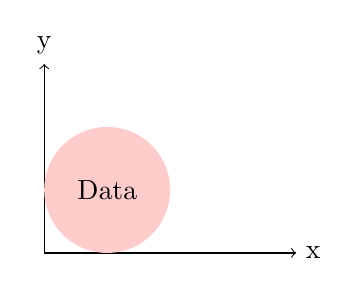
\begin{tikzpicture}[scale=0.8]
\draw[->] (0,0) -- (4,0) node[right] {x};
\draw[->] (0,0) -- (0,3) node[above] {y};
\fill[red!20] (1,1) circle (1);
\node at (1,1) {Data};
\end{tikzpicture}
\end{center}

\end{column}
%
\begin{column}{.33\textwidth}

\block{Results}
Presentation of research results.

\alertblock{Alert Block}
Important findings or warnings.

\block{Conclusion}
Summary and conclusions of the research.

\end{column}
\end{columns}

\begin{columns}
\begin{column}{.7\textwidth}

\block{References}
\begin{thebibliography}{9}
\bibitem{ref1} Author, A. (2023). Title. Journal, Volume(Issue), Pages.
\bibitem{ref2} Researcher, B. (2022). Book Title. Publisher.
\end{thebibliography}

\end{column}
%
\begin{column}{.3\textwidth}

\block{Contact}
Ostap S. Bender \\
RUDN University \\
email@example.com

\end{column}
\end{columns}

\end{frame}

\end{document}
\end{verbatim}

\subsection*{Generated figure}
Poster using beamerposter package.

\subsection*{Screenshot}
\begin{center}
\includegraphics[width=0.8\textwidth]{772PresentationBeamerPoster.png}
\end{center}

\vspace{20pt}\hrule\vspace{20pt}

% ============================================================
\section{773PresentationTikZPoster1 - TikZPoster with Errors}
\label{sec:773a}

\begin{verbatim}
\documentclass[25pt, a0paper, portrait]{tikzposter} % 25pt est une taille standard pour A0
\usepackage[utf8]{inputenc}

\usetheme{Board} % Thème standard 
\title{Boltzmann's entropy} % Correction orthographe 'entropy'
\author{TETE PELE}
\institute{RUDN University}

\begin{document}
  \maketitle

  \begin{columns}
    \column{.33}
      \block{MONGE Gaspard}{Definition and Development: 1st column definition of transport}

    \column{.33}
      \block{Richi}{Definition and Development: Geometrics definition}

    \column{.33}
      \block{Kantorovich}{Definition and Development: Transformation in Linear problems}
  \end{columns}

  \block{Conclusion}{Synthèse avec Cédric V.}

\end{document}


\documentclass[24pt, a0paper, portrait]{tikzposter}% begin the TikZ
\usepackage[multicol]

\usetheme{Transport theory}
\title{Boltzmann's antropie}
\author{TETE PELE}
\institute{RUDN University}

\begin{document}
  \maketitle
   Transport theory
\begin{columns}% 
  \column{.33}{MONGE Gaspard}{ Definition and Developpment}
1st column definition of transport 
  \column{.33}
   Richi 
  \Section{ Definition and Developpment}
Geometics definition
  \column{.33}
    Kantarovich
  \Section{ Definition and Developpment}
Transfortion in Lineare probleme
\end{columns}
%Synthese with Cedric V
\begin{columns}
Conclusion
\end{columns}

\end{document}
\end{verbatim}

\subsection*{Generated figure}
TikZPoster with corrected and incorrect versions.

\subsection*{Screenshot}
\begin{center}
\includegraphics[width=0.8\textwidth]{773PresentationTikZPoster1.png}
\end{center}

\vspace{20pt}\hrule\vspace{20pt}

% ============================================================
\section{773PresentationTikZPoster2 - TikZPoster}
\label{sec:773b}

\begin{verbatim}
\documentclass[24pt, a0paper, portrait]{tikzposter}
\usepackage[utf8]{inputenc}
\usepackage[T1]{fontenc}
\usepackage{multicol}
\usepackage{graphicx}
\usepackage{tikz}
\usepackage{caption}
\usepackage{color}

\definecolor{MyPink}{RGB}{194, 19, 182}
\definecolor{MyBlue}{RGB}{30, 100, 200}
\definecolor{MyGreen}{RGB}{50, 150, 100}

\usetheme{Default}

\title{Look I'm making a poster}
\author{Ostap S. Bender}
\institute{RUDN University}

\begin{document}

\maketitle

\begin{columns}
\column{.33}

\block{Introduction}{
This is the introduction section. Here follows some regular text, \color{MyPink} from now on the text has changed colour, \color{black} and then we are back to normal.
\vspace{3cm}
}
\note[targetoffsetx=-11cm, targetoffsety=-6.5cm, width=10cm]{This is an important note about the introduction}

\begin{center}
\includegraphics[width=0.9\colwidth]{faucon.jpg}
\captionof{figure}{faucon.jpg}
\end{center}

\column{.33}

\block{Methods}{
Details about the methodology used in this research.
}

\begin{center}
\begin{tikzpicture}[scale=0.7]
\draw[->, thick] (0,0) -- (5,0) node[right] {Time};
\draw[->, thick] (0,0) -- (0,4) node[above] {Value};
\draw[MyBlue, very thick] plot[domain=0:4.5, samples=50] (\x, {1.5 + sin(\x*100)});
\draw[MyGreen, very thick] plot[domain=0:4.5, samples=50] (\x, {2.5 + 0.5*cos(\x*120)});
\node[MyBlue] at (2,3.5) {Method A};
\node[MyGreen] at (3,1.5) {Method B};
\end{tikzpicture}
\captionof{figure}{Comparison of methods}
\end{center}

\column{.33}

\block{Results}{
Presentation of research results and findings.
}

\block{Conclusion}{
Summary and conclusions of the research. Key findings and future work.
}

\end{columns}

\begin{columns}
\column{.7}

\block{References}{
\begin{multicols}{2}
\begin{thebibliography}{9}
\bibitem{ref1} Author, A. (2023). Title. Journal, Volume(Issue), Pages.
\bibitem{ref2} Researcher, B. (2022). Book Title. Publisher.
\bibitem{ref3} Scientist, C. (2021). Conference Proceedings.
\bibitem{ref4} Scholar, D. (2020). Technical Report.
\end{thebibliography}
\end{multicols}
}

\column{.3}

\block{Contact Information}{
\textbf{Ostap S. Bender} \\
RUDN University \\
Department of Mathematics \\
\texttt{email@rudn.ru} \\
+7 (906) 000-00-00
}

\block{Acknowledgements}{
This research was supported by RUDN University.
}

\end{columns}

\end{document}
\end{verbatim}

\subsection*{Generated figure}
Complete TikZPoster with colors, figures, and proper structure.

\subsection*{Screenshot}
\begin{center}
\includegraphics[width=0.9\textwidth]{773PresentationTikZPoster2.png}
\end{center}

\vspace{20pt}\hrule\vspace{20pt}

\section*{Conclusion: Methodology for creating successful Beamer and Poster presentations}
\addcontentsline{toc}{section}{Conclusion}

After exhaustive study of Beamer and Poster examples, here is the structured methodology for creating successful presentations:

\subsection*{1. Essential basic structure for Beamer}
\begin{verbatim}
\documentclass{beamer}
\usetheme{ThemeName}          % Choose a theme
\usecolortheme{ColorTheme}    % Optional color theme
\title{Presentation Title}
\author{Your Name}
\date{\today}
\begin{document}
\begin{frame}
\titlepage
\end{frame}
\begin{frame}{Frame Title}
% Content here
\end{frame}
\end{document}
\end{verbatim}

\subsection*{2. Essential basic structure for TikZPoster}
\begin{verbatim}
\documentclass[24pt, a0paper, portrait]{tikzposter}
\usepackage[utf8]{inputenc}
\usepackage{graphicx}
\usepackage{tikz}
\usetheme{Default}
\title{Poster Title}
\author{Your Name}
\institute{Your Institution}
\begin{document}
\maketitle
\begin{columns}
\column{.33}
\block{Section Title}{
Content here
}
\end{columns}
\end{document}
\end{verbatim}

\subsection*{3. Recommended progressive approach}
\textbf{Step 1: Planning}
\begin{itemize}
\item Define presentation structure (title, sections, content)
\item Choose appropriate theme and colors
\item Prepare visual elements (images, diagrams)
\end{itemize}

\textbf{Step 2: Build in layers}
\begin{enumerate}
\item Basic structure (title page, sections)
\item Content (text, blocks, items)
\item Visual elements (images, TikZ graphics)
\item Animations and overlays (pause, uncover)
\item Final polish (notes, references)
\end{enumerate}

\textbf{Step 3: Optimize}
\begin{itemize}
\item Use consistent formatting
\item Balance text and visuals
\item Test on different screen sizes (for presentations)
\item Check printability (for posters)
\end{itemize}

\subsection*{4. Essential best practices}
\begin{tabular}{|l|l|}
\hline
\textbf{Practice} & \textbf{Example} \\
\hline
Use appropriate themes & \texttt{\textbackslash usetheme\{Copenhagen\}} \\
Organize with blocks & \texttt{\textbackslash begin\{block\}\{Title\}...\textbackslash end\{block\}} \\
Add visual elements & Images, TikZ diagrams \\
Use overlays effectively & \texttt{\textbackslash pause}, \texttt{\textbackslash uncover} \\
Maintain consistency & Same fonts, colors, sizes \\
\hline
\end{tabular}

\subsection*{5. Synthetic conclusion}
\begin{framed}
\textbf{To create successful presentations:}

1. \textbf{Structure}: Title → Introduction → Content → Conclusion → References

2. \textbf{Visuals}: Balance text and graphics, use consistent theme

3. \textbf{Animation}: Use \texttt{pause} and \texttt{uncover} for stepwise revelation

4. \textbf{Posters}: Use appropriate classes (tikzposter, a0poster, beamerposter)

5. \textbf{Testing}: Compile frequently, test on target display/print

\end{framed}

\vspace{10pt}
\textbf{Final reminder}: Beamer and poster creation tools are powerful for academic communication. Start with simple templates, gradually add complexity, and always prioritize clarity and readability over visual effects.

\end{document}